\documentclass[a4paper]{article}

%% Language and font encodings
\usepackage[english]{babel}
\usepackage[utf8x]{inputenc}
\usepackage[T1]{fontenc}

%% Sets page size and margins
\usepackage[a4paper,top=3cm,bottom=2cm,left=3cm,right=3cm,marginparwidth=1.75cm]{geometry}

%% Useful packages
\usepackage{amsmath}
\usepackage{graphicx}
\usepackage[colorinlistoftodos]{todonotes}
\usepackage[colorlinks=true, allcolors=blue]{hyperref}

\title{Real-Time Systems Lab 2}
\author{Niklas Hollenbeck (735992), Lukas Giesler (741676)}
\date{}
\begin{document}
\maketitle

\section{Timeline output as String for RMS and DMS}
\begin{center}
	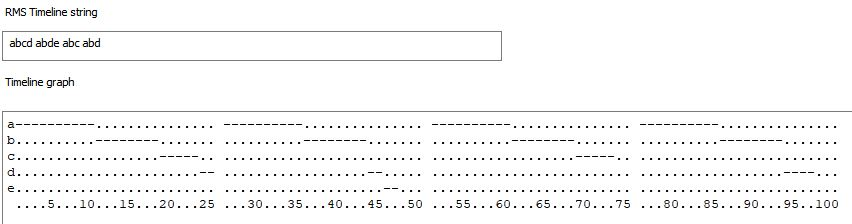
\includegraphics[width=450px]{img1.JPG}
\end{center}

\section{Response Time Analysis}
\begin{center}
	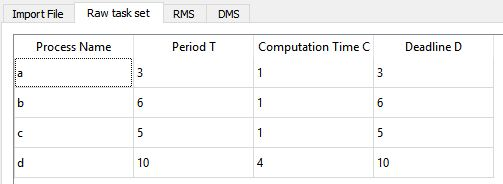
\includegraphics[width=350px]{img4.JPG}
\end{center}

\subsection{Simplified RTA}
\begin{center}
	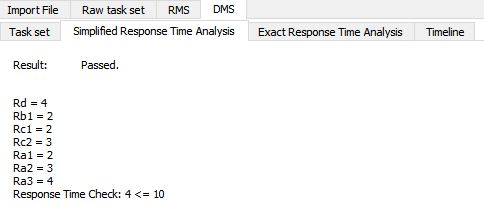
\includegraphics[width=350px]{img2.JPG}
\end{center}

\subsection{Exact RTA}
\begin{center}
	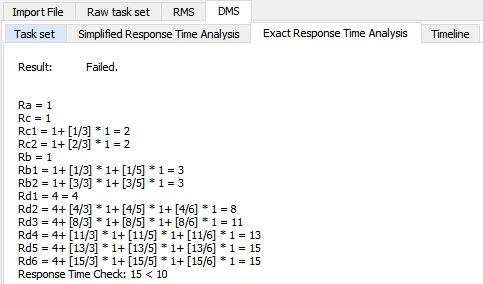
\includegraphics[width=350px]{img3.JPG}
\end{center}

\subsection{Comparing the Results}
It's clear that the simplified RTA has shown a significantly different result in this example. While the simplified RTA evaluated that the analysis was passed successfully, the exact RTA evaluated that this task failed the analysis.

\section{Optimal Priority Assignment using Exact RTA}
\subsection{Before OPA, Priority assigned by order}
\begin{center}
	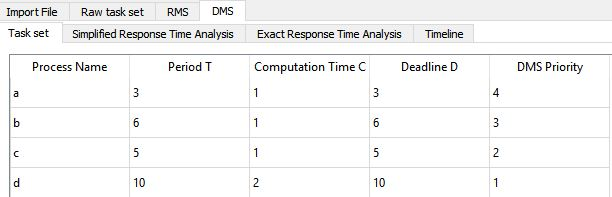
\includegraphics[width=350px]{img5.JPG}
\end{center}
\subsection{After OPA}
\begin{center}
	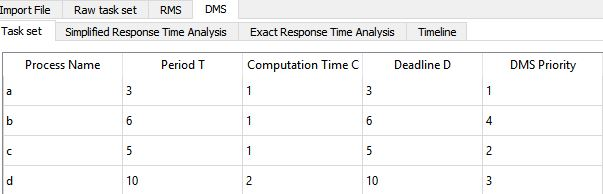
\includegraphics[width=350px]{img6.JPG}
\end{center}

\end{document}